% SVN info for this file
\svnidlong
{$HeadURL$}
{$LastChangedDate$}
{$LastChangedRevision$}
{$LastChangedBy$}

\chapter{Topologia quoziente}
\labelChapter{topologia quoziente}

\begin{introduction}
‘‘BEEP BOOP INSERIRE CITAZIONE QUA BEEP BOOP.''
\begin{flushright}
	\textsc{NON UN ROBOT,} UN UMANO IN CARNE ED OSSA BEEP BOOP.
\end{flushright}
\end{introduction}

		\section{Topologia Quoziente}
%AAA INTRODUZIONE BELLA CERCASI
Torniamo ora a parlare di costruzioni topologiche, in particolare ci domandiamo quale sia la topologia più adatta per un insieme quoziente. Ne diamo prima una definizione come topologia indotta da una funzione fra uno spazio topologico ed un insieme, poi vedremo altre definizioni equivalenti tramite una funzione fra spazi topologici e con insiemi quozienti.\newline
Accenniamo fin da subito che la situazione è \textit{duale} rispetto a quella dei sottospazi, analizzati nella sezione 
%AAA SEZIONE CERCASI
\begin{define}
	Dato $X$ uno spazio topologico, $Y$ un \textit{insieme} e $\funz f X Y$ funzione suriettiva, la \textbf{topologia quoziente} su $Y$ indotta da $f$ è la topologia \textit{più fine} che rende $f$ continua.
\end{define}
Analizziamo ora chi sono i suoi aperti: $\displaystyle A\subseteq Y \text{ aperto } \iff f^{-1}(A)\subseteq X$ aperto. Notiamo che l'implicazione $\Rightarrow)$ è necessaria perchè $f$ sia continua, mentre l'implicazione $\Leftarrow)$ è quella che caratterizza la topologia quoziente, infatti se si considera un insieme $B\subseteq Y$ che non è aperto allora la sua controimmagine $f^{-1}(B)\subseteq X$ non sarà aperta, dunque la topologia su $Y$ è la più fine.\newline
%AAA NUOVO ENVIRONMENT CERCASI
Per verificare che un sottoinsieme sia aperto in $Y$ con la topologia quoziente bisogna verificare che la sua controimmagine è aperta.

Vediamo ora un esempio che giustifica la terminologia "topologia quoziente".
\begin{example}
	Sia $X$ uno spazio topologico e $\sim$ una relazione di equivalenza su $X$. Posto $Y=\nicefrac{X}{\sim}$ insieme quoziente e $\funztot \pi X Y x {[x]_\sim}$ proiezione al quoziente, la topologia quoziente su $Y$ è quella che rende la proiezione continua.
\end{example}


Ricordiamo il primo teorema fondamentale di isomorfismo per gli \textit{insiemi}, altresì chiamato decomposizione canonica.\newline
	\begin{minipage}[t]{0.83\textwidth}
		Data una qualsiasi funzione suriettiva $\funz f X Y$ vi è la seguente relazione di equivalenza: $\displaystyle \forall x,y\in X, \ x\sim y \iff f(x)=f(y)$, inoltre $\exists ! \funz h {\nicefrac{X}{\sim}} Y$ biunivoca tale che $f=h\circ\pi$, baste porre $h\left( [x] \right) \coloneqq f(x)$, in modo tale che il diagramma commuti. Mostriamo che è ben definita e biunivoca.
	\end{minipage}
	\begin{minipage}[t]{0.13\textwidth}\vspace{-10pt}
		\begin{tikzcd}
			X \arrow[r, "f"] \arrow[d, "\pi"']                                   & Y \\
			\nicefrac{X}{\sim} \arrow[ru, "\exists !h"', dotted] &    
		\end{tikzcd}
	\end{minipage}
	\begin{gather*}
		[x]=[y]\iff x\sim t\iff f(x)=f(y)\iff h([x])=h([y]) \implies h \text{ ben definita e iniettiva }\\
		f \text{ suriettiva } \implies h \text{ suriettiva}
	\end{gather*}

	\subsection{Identificazione}
Tenendo a mente il concetto di immersione illustrato a pagina \pageref{immersione} illustriamo il concetto duale di identificazione.
\begin{define}
	Siano $X,Y$ spazi topologici e $\funz f X Y$ una funzione continua e suriettiva; $f$ si dice \textbf{identificazione} se $Y$ ha la topologia quoziente indotta da $f$.
\end{define}
In generale è difficile determinare quando una data funzione è un'identificazione, quindi ne cerchiamo una condizione sufficiente. 
%CONFUSIONE TIME: è sufficiente o necessaria?
\begin{theorema} \textsc{Manetti, 5.4}\\
	Sia $\funz f X Y$continua, suriettiva e chiusa (o aperta), alora $f$ è un'identificazione chiusa (o aperta).
\end{theorema}
\begin{demonstration}
	Supponiamo che $f$ sia aperta. Dimostrare che è un'identificazione è equivalente al mostrare che $\displaystyle A\subseteq Y \text{ aperto } \iff f^{-1}(A)\subseteq X$ aperto. L'implicazione $\Rightarrow)$ è garantita dalla continuità di $f$, per quanto riguarda l'implicazione opposta $\Leftarrow)$ invece siccome $f$ è suriettiva allora $f(f^{-1}(A))=A$ e siccome $f$ è aperta allora anche $A$ è aperto.
\end{demonstration}

Vediamo ora un esempio di identificazione chiusa e non aperta.
%POTREBBE STARCI UN DISEGNO?
\begin{example}
% FRECCIA CHE NON ARRIVA A DESTINAZIONE
	Si consideri $\displaystyle \funztot f {[0, \ 2\pi]} {S^1} t {(\cos t, \ \sin t)}$. è una funzione continua, suriettiva e chiusa (compatto in $T_2$), dunque è un'identificazione chiusa. \\
	Tuttavia $f$ non è aperta, infatti dato $A=[0, \ 1)\subseteq [0, \ 2\pi]$ aperto, ma $f(A)$ non è aperto in $S^1$.
%RICKROLL
		\begin{center}
			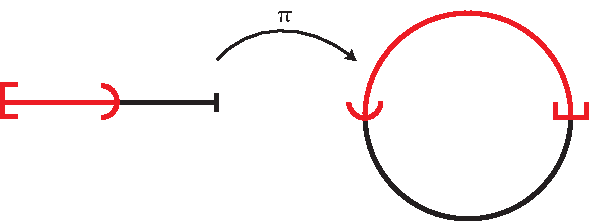
\includegraphics[width=240pt]{images/half_circle-eps-converted-to}
		\end{center}
\end{example}

\begin{observe}
	Gli omeomorfismi sono identificazioni chiuse e aperte.
\end{observe}

Vediamo ora che relazione c'è fra le identificazioni ed i quozienti dati da relazioni di equivalenza.
\begin{theorema} \textsc{proprietà universale delle identificazioni, Manetti, 5.6} \\
	\begin{minipage}[t]{0.83\textwidth}
		Dati $X,Y,Z$ spazi topologici, $g$ una qualsiasi funzione continua, \\
		$f$ identificazione con le mappe come in figura, allora \\
		$\exists ! h \text{ continua } \colon g=h\circ f \iff \left( \forall x,y\in X, \ f(x)=f(y)\implies g(x)=g(y)  \right)$ \\
		ovvero se e solo se $g$ è costante sulle fibre di $f$.
	\end{minipage}
	\begin{minipage}[t]{0.13\textwidth}\vspace{-10pt}
		\begin{tikzcd}
			X \arrow[r, "f"] \arrow[d, "g"']                                   & Y \\
			Z \arrow[ur, "\exists !h"', dotted] &    
		\end{tikzcd} 
%LA FRECCIA è AL CONTRARIO
	\end{minipage}
\end{theorema}
\begin{demonstration}
	Idealmente se $f$ fosse invertibile definiremmo $h=g\circ f^{-1}$. Tuttavia l'invertibilità di $f$ non è fra le ipotesi, quindi si sfrutta al meglio l'ipotesi della suriettività e si considera una controimmagine tramite $f$ e se ne fa l'immagine tramite $g$, ovvero $y\in Y, \ h(y)\coloneqq g(x)$ con $x\in f^{-1}(y)$. Con questa costruzione $h$ è ben definita siccome $g$ sarà costante sulle fibre di $f$. \\
	Verifichiamo che $h$ è continua tramite la definizione:
		\begin{gather*}
			U\subseteq Z \text{ aperto }, \ h^{-1}(U)\subseteq Y \iff f^{-1}(h^{-1}(U))\subseteq X \text{ aperto} \iff g^{-1}(U)\subseteq X \text{ aperto}
		\end{gather*}
	Siccome $g$ è continua allora lo è anche $h$.
\end{demonstration}

%QUESTO DISCORSETTO CARINO ED IMPORTANTE LO DEVO METTERE IN UN ENVIRONMENT?
%SENZA ENVIRONMENT SBORDA ED INIZIA PIù A DESTRA
	\begin{minipage}[t]{0.83\textwidth}
		Come conseguenza si ha che data $f$ continua, $\sim$ relazione di equivalenza e $\nicefrac{X}{\sim}$ spazio topologico con la topologia quoziente indotta dalla proiezione $\pi$ si ha che $\exists g$ continua $\iff \left( x\sim y \implies f(x)=f(y) \right)$, ovvero $\pi$ è costante sulle fibre di $f$.
	 	\end{minipage}
 	\begin{minipage}[t]{0.13\textwidth}\vspace{-10pt}
 		\begin{tikzcd}
		 	X \arrow[r, "f"] \arrow[d, "\pi"']                                   & Y \\
 			\nicefrac{X}{\sim} \arrow[ur, "g"', dotted] &    
		\end{tikzcd}
	\end{minipage}
	\begin{minipage}[t]{0.83\textwidth}
		In particolare se $f$ è la relazione d'equivalenza indotta da $f$, ovvero se si è nelle ipotesi del primo teorema fondamentale di isomorfismo degli insiemi allora $\left( x\sim y \iff f(x)=f(y) \right) \implies \exists ! \overline{f}$ biettiva, continua. Dunque vale 
			\begin{equation}
				\overline{f} \text{ omeomorfismo} \iff f \text{ identificazione}
			\end{equation}
	 	\end{minipage}
		\begin{minipage}[t]{0.13\textwidth}\vspace{-10pt}
			\begin{tikzcd}
				X \arrow[r, "f"] \arrow[d, "\pi"']                                   & Y \\
				\nicefrac{X}{\sim} \arrow[ur, "\overline{f}"', dotted] &    
			\end{tikzcd}
		\end{minipage}\\
	
Riprendiamo l'esempio precedente ed esaminiamolo in termini di spazio quoziente.
\begin{example}~{$\nicefrac{D^n}{\sim}\cong S^n$}\\
	$\funztot f {D^1=[0, \ 2\pi]} {S^1} t {(\cos t, \ \sin t)}, \ \ f$ 
%FRECCIA CHE NON ARRIVA A DESTINAZIONE	
	identificazione $\implies S^!\cong \nicefrac{[0, \ 2\pi]}{\sim}$, con $\sim$ tale che sia costante sulle fibre di $f$: $\displaystyle s\sim t \iff \begin{cases} 
		\cos s=\cos t \\
		\sin s =\sin t
	\end{cases} \iff s=t$ oppure $s=0,\ t=2\pi$ \newline
	Si può generalizzare in dimensione $n$ con $\funztot f {D^n} {S^n} x {\left( 2x\sqrt{1- \| x \|^2}, \ 2\| x\|^2 -1 \right)}$ identificazione, dunque $\nicefrac{D^n}{\sim}\cong S^n$ per la relazione $(x_1,\ y_1) \sim (x_2,\ y_2)\iff \begin{cases}
		(x_1,\ y_1)=(x_2,\ y_2)\\
		x_1^2 +y_1^2= x_2^2 +y_2^2=1
	\end{cases}$ ovvero ogni punto è in relazione con sé stesso e tutti i punti sul bordo sono identificati.
\end{example}
	
%LEZ 12
	\subsection{Quozienti tipici}
Vedremo ora degli esempi di spazi quoziente usati frequentemente.
\subsubsection{Contrazione di $A$ ad un punto}
Sia $X$ uno spazio topologico, $A\subseteq X$, $\forall x,y\in X \ x\sim y\iff x=y$ oppure $x,y\in A$, ovvero ogni punto è in relazione con sé stesso e tutti i punti di $A$ sono in relazione fra loro, dunque quozientando si "contraggono" ad un unico punto.
\begin{example} $\nicefrac{D^n}{S^{n-1}}\cong S^n$ \\
	Cerchiamo ora di generalizzare l'esempio precedente. Ricordiamo che relazione c'è fra i dischi e le sfere:
		\begin{gather*}
			D^n=\text{ disco in } \realset^n=\{x\in\realset^n \mid \| x \| \leq 1 \}\\
			S^{n-1}=\text{ bordo di } D^n=\{x\in\realset^n \mid \| x \| = 1 \}
		\end{gather*}
	Considerando $\sim$ come la contrazione di $S^{n-1}$ ad un punto, si ha che $\nicefrac{D^n}{S^{n-1}} \cong S^n$	
\end{example}

\begin{attention}
	Anche se $X$ è $T_2$ non è detto che $\nicefrac{X}{A}$ è $T_2$!\newline
	Se $A$ non è chiuso allora $\nicefrac{X}{A}$ non è neanche $T_1$, infatti $\pi^{-1}([A])=A$ non chiuso implica che $[A]$ non lo è, quindi per la caratterizzazione degli spazi $T_1$ (vedasi %AAA TEOREMA CERCASI) 
	$\nicefrac{X}{A}$ non è $T_1$.\newline 
	Tuttavia se $X$ è $T_2$, $K\subseteq X$ è compatto allora $\nicefrac{X}{K}$ è $T_2$
\end{attention}

\subsubsection{Cono su uno spazio}
\begin{define}
	Sia $X$ uno spazio topologico, si definisce \textbf{cilindro} su $X$ lo spazio $X\times \intv$.\newline 
	Il \textbf{cono} su $X$ invece è il quoziente $\displaystyle \nicefrac{X\times\intv}{X\times\{1\}}$ oppure $\displaystyle \nicefrac{X\times\intv}{X\times\{0\}}$.
\end{define}

\begin{observe}
	Un cono è sempre c.p.a. rispetto al "vertice".
\end{observe}